\documentclass[]{article}
\usepackage{lmodern}
\usepackage{amssymb,amsmath}
\usepackage{ifxetex,ifluatex}
\usepackage{fixltx2e} % provides \textsubscript
\ifnum 0\ifxetex 1\fi\ifluatex 1\fi=0 % if pdftex
  \usepackage[T1]{fontenc}
  \usepackage[utf8]{inputenc}
\else % if luatex or xelatex
  \ifxetex
    \usepackage{mathspec}
  \else
    \usepackage{fontspec}
  \fi
  \defaultfontfeatures{Ligatures=TeX,Scale=MatchLowercase}
\fi
% use upquote if available, for straight quotes in verbatim environments
\IfFileExists{upquote.sty}{\usepackage{upquote}}{}
% use microtype if available
\IfFileExists{microtype.sty}{%
\usepackage{microtype}
\UseMicrotypeSet[protrusion]{basicmath} % disable protrusion for tt fonts
}{}
\usepackage[margin=1in]{geometry}
\usepackage{hyperref}
\hypersetup{unicode=true,
            pdfborder={0 0 0},
            breaklinks=true}
\urlstyle{same}  % don't use monospace font for urls
\usepackage{color}
\usepackage{fancyvrb}
\newcommand{\VerbBar}{|}
\newcommand{\VERB}{\Verb[commandchars=\\\{\}]}
\DefineVerbatimEnvironment{Highlighting}{Verbatim}{commandchars=\\\{\}}
% Add ',fontsize=\small' for more characters per line
\usepackage{framed}
\definecolor{shadecolor}{RGB}{248,248,248}
\newenvironment{Shaded}{\begin{snugshade}}{\end{snugshade}}
\newcommand{\KeywordTok}[1]{\textcolor[rgb]{0.13,0.29,0.53}{\textbf{#1}}}
\newcommand{\DataTypeTok}[1]{\textcolor[rgb]{0.13,0.29,0.53}{#1}}
\newcommand{\DecValTok}[1]{\textcolor[rgb]{0.00,0.00,0.81}{#1}}
\newcommand{\BaseNTok}[1]{\textcolor[rgb]{0.00,0.00,0.81}{#1}}
\newcommand{\FloatTok}[1]{\textcolor[rgb]{0.00,0.00,0.81}{#1}}
\newcommand{\ConstantTok}[1]{\textcolor[rgb]{0.00,0.00,0.00}{#1}}
\newcommand{\CharTok}[1]{\textcolor[rgb]{0.31,0.60,0.02}{#1}}
\newcommand{\SpecialCharTok}[1]{\textcolor[rgb]{0.00,0.00,0.00}{#1}}
\newcommand{\StringTok}[1]{\textcolor[rgb]{0.31,0.60,0.02}{#1}}
\newcommand{\VerbatimStringTok}[1]{\textcolor[rgb]{0.31,0.60,0.02}{#1}}
\newcommand{\SpecialStringTok}[1]{\textcolor[rgb]{0.31,0.60,0.02}{#1}}
\newcommand{\ImportTok}[1]{#1}
\newcommand{\CommentTok}[1]{\textcolor[rgb]{0.56,0.35,0.01}{\textit{#1}}}
\newcommand{\DocumentationTok}[1]{\textcolor[rgb]{0.56,0.35,0.01}{\textbf{\textit{#1}}}}
\newcommand{\AnnotationTok}[1]{\textcolor[rgb]{0.56,0.35,0.01}{\textbf{\textit{#1}}}}
\newcommand{\CommentVarTok}[1]{\textcolor[rgb]{0.56,0.35,0.01}{\textbf{\textit{#1}}}}
\newcommand{\OtherTok}[1]{\textcolor[rgb]{0.56,0.35,0.01}{#1}}
\newcommand{\FunctionTok}[1]{\textcolor[rgb]{0.00,0.00,0.00}{#1}}
\newcommand{\VariableTok}[1]{\textcolor[rgb]{0.00,0.00,0.00}{#1}}
\newcommand{\ControlFlowTok}[1]{\textcolor[rgb]{0.13,0.29,0.53}{\textbf{#1}}}
\newcommand{\OperatorTok}[1]{\textcolor[rgb]{0.81,0.36,0.00}{\textbf{#1}}}
\newcommand{\BuiltInTok}[1]{#1}
\newcommand{\ExtensionTok}[1]{#1}
\newcommand{\PreprocessorTok}[1]{\textcolor[rgb]{0.56,0.35,0.01}{\textit{#1}}}
\newcommand{\AttributeTok}[1]{\textcolor[rgb]{0.77,0.63,0.00}{#1}}
\newcommand{\RegionMarkerTok}[1]{#1}
\newcommand{\InformationTok}[1]{\textcolor[rgb]{0.56,0.35,0.01}{\textbf{\textit{#1}}}}
\newcommand{\WarningTok}[1]{\textcolor[rgb]{0.56,0.35,0.01}{\textbf{\textit{#1}}}}
\newcommand{\AlertTok}[1]{\textcolor[rgb]{0.94,0.16,0.16}{#1}}
\newcommand{\ErrorTok}[1]{\textcolor[rgb]{0.64,0.00,0.00}{\textbf{#1}}}
\newcommand{\NormalTok}[1]{#1}
\usepackage{graphicx,grffile}
\makeatletter
\def\maxwidth{\ifdim\Gin@nat@width>\linewidth\linewidth\else\Gin@nat@width\fi}
\def\maxheight{\ifdim\Gin@nat@height>\textheight\textheight\else\Gin@nat@height\fi}
\makeatother
% Scale images if necessary, so that they will not overflow the page
% margins by default, and it is still possible to overwrite the defaults
% using explicit options in \includegraphics[width, height, ...]{}
\setkeys{Gin}{width=\maxwidth,height=\maxheight,keepaspectratio}
\IfFileExists{parskip.sty}{%
\usepackage{parskip}
}{% else
\setlength{\parindent}{0pt}
\setlength{\parskip}{6pt plus 2pt minus 1pt}
}
\setlength{\emergencystretch}{3em}  % prevent overfull lines
\providecommand{\tightlist}{%
  \setlength{\itemsep}{0pt}\setlength{\parskip}{0pt}}
\setcounter{secnumdepth}{0}
% Redefines (sub)paragraphs to behave more like sections
\ifx\paragraph\undefined\else
\let\oldparagraph\paragraph
\renewcommand{\paragraph}[1]{\oldparagraph{#1}\mbox{}}
\fi
\ifx\subparagraph\undefined\else
\let\oldsubparagraph\subparagraph
\renewcommand{\subparagraph}[1]{\oldsubparagraph{#1}\mbox{}}
\fi

%%% Use protect on footnotes to avoid problems with footnotes in titles
\let\rmarkdownfootnote\footnote%
\def\footnote{\protect\rmarkdownfootnote}

%%% Change title format to be more compact
\usepackage{titling}

% Create subtitle command for use in maketitle
\newcommand{\subtitle}[1]{
  \posttitle{
    \begin{center}\large#1\end{center}
    }
}

\setlength{\droptitle}{-2em}
  \title{}
  \pretitle{\vspace{\droptitle}}
  \posttitle{}
  \author{}
  \preauthor{}\postauthor{}
  \date{}
  \predate{}\postdate{}


\begin{document}

{
\setcounter{tocdepth}{1}
\tableofcontents
}
\subsubsection{Correlation}\label{correlation}

Correlaton refers to the strength of the relationship between two
different variables.

Correlation is often represented by the letter r.

The equation for correlation(r) looks a little intimidating but if it is
broken down into steps, it is much more managable.

\(r = \frac{n(\sum(xy)-(\sum x)(\sum(y))}{\sqrt{n \sum x ^2-(\sum x)^2][n \sum y ^2-(\sum y)^2]}}\)

Let's take a closer look at the denominator first:

\begin{enumerate}
\def\labelenumi{\arabic{enumi}.}
\tightlist
\item
  \(n(\sum(xy)-(\sum x)(\sum(y))\)
\end{enumerate}

The first thing we should do is have a dataset to work with:

x = 5, 5, 4, 4, 5, 5, 4, 5, 3, 5, 6, 6, 5, 6, 6 y = 13, 12, 13, 14, 13,
12, 11, 12, 11, 12, 13, 12, 12, 13, 13

Each dataset has 15 data points. When you work with larger datasets you
may want to avoid having to count each number so r has a built in
function called \texttt{length()} which will return the number of items
in your variable. We know our first term is 15 so we will add that to
the formula.

\begin{enumerate}
\def\labelenumi{\arabic{enumi}.}
\setcounter{enumi}{1}
\tightlist
\item
  \(r = \frac{15(\sum(xy)-(\sum x)(\sum(y))}{\sqrt{15 \sum x ^2-(\sum x)^2][15 \sum y ^2-(\sum y)^2]}}\)
\end{enumerate}

The next part is asking us to compute the sum of the values of x
multiplied by the values of y and then add that to the formula.

\begin{Shaded}
\begin{Highlighting}[]
\NormalTok{x =}\StringTok{ }\KeywordTok{c}\NormalTok{(}\DecValTok{5}\NormalTok{, }\DecValTok{5}\NormalTok{, }\DecValTok{4}\NormalTok{, }\DecValTok{4}\NormalTok{, }\DecValTok{5}\NormalTok{, }\DecValTok{5}\NormalTok{, }\DecValTok{4}\NormalTok{, }\DecValTok{5}\NormalTok{, }\DecValTok{3}\NormalTok{, }\DecValTok{5}\NormalTok{, }\DecValTok{6}\NormalTok{, }\DecValTok{6}\NormalTok{, }\DecValTok{5}\NormalTok{, }\DecValTok{6}\NormalTok{, }\DecValTok{6}\NormalTok{)}
\NormalTok{y =}\StringTok{ }\KeywordTok{c}\NormalTok{(}\DecValTok{13}\NormalTok{, }\DecValTok{12}\NormalTok{, }\DecValTok{13}\NormalTok{, }\DecValTok{14}\NormalTok{, }\DecValTok{13}\NormalTok{, }\DecValTok{12}\NormalTok{, }\DecValTok{11}\NormalTok{, }\DecValTok{12}\NormalTok{, }\DecValTok{11}\NormalTok{, }\DecValTok{12}\NormalTok{, }\DecValTok{13}\NormalTok{, }\DecValTok{12}\NormalTok{, }\DecValTok{12}\NormalTok{, }\DecValTok{13}\NormalTok{, }\DecValTok{13}\NormalTok{)}
\NormalTok{xy=}\KeywordTok{sum}\NormalTok{(x}\OperatorTok{*}\NormalTok{y)}
\NormalTok{xy}
\end{Highlighting}
\end{Shaded}

\begin{verbatim}
## [1] 921
\end{verbatim}

\begin{enumerate}
\def\labelenumi{\arabic{enumi}.}
\setcounter{enumi}{2}
\tightlist
\item
  \(r = \frac{15(921)-(\sum x)(\sum(y))}{\sqrt{15 \sum x ^2-(\sum x)^2][15 \sum y ^2-(\sum y)^2]}}\)
\end{enumerate}

Next we need to subtract this amount from the result from the product of
the sum of all of the values of x and the sum of all the values of y.

\begin{Shaded}
\begin{Highlighting}[]
\NormalTok{x =}\StringTok{ }\KeywordTok{c}\NormalTok{(}\DecValTok{5}\NormalTok{, }\DecValTok{5}\NormalTok{, }\DecValTok{4}\NormalTok{, }\DecValTok{4}\NormalTok{, }\DecValTok{5}\NormalTok{, }\DecValTok{5}\NormalTok{, }\DecValTok{4}\NormalTok{, }\DecValTok{5}\NormalTok{, }\DecValTok{3}\NormalTok{, }\DecValTok{5}\NormalTok{, }\DecValTok{6}\NormalTok{, }\DecValTok{6}\NormalTok{, }\DecValTok{5}\NormalTok{, }\DecValTok{6}\NormalTok{, }\DecValTok{6}\NormalTok{)}
\NormalTok{y =}\StringTok{ }\KeywordTok{c}\NormalTok{(}\DecValTok{13}\NormalTok{, }\DecValTok{12}\NormalTok{, }\DecValTok{13}\NormalTok{, }\DecValTok{14}\NormalTok{, }\DecValTok{13}\NormalTok{, }\DecValTok{12}\NormalTok{, }\DecValTok{11}\NormalTok{, }\DecValTok{12}\NormalTok{, }\DecValTok{11}\NormalTok{, }\DecValTok{12}\NormalTok{, }\DecValTok{13}\NormalTok{, }\DecValTok{12}\NormalTok{, }\DecValTok{12}\NormalTok{, }\DecValTok{13}\NormalTok{, }\DecValTok{13}\NormalTok{)}
\NormalTok{sumx =}\StringTok{ }\KeywordTok{sum}\NormalTok{(x)}
\NormalTok{sumy =}\StringTok{ }\KeywordTok{sum}\NormalTok{(y)}
\NormalTok{sumx}
\end{Highlighting}
\end{Shaded}

\begin{verbatim}
## [1] 74
\end{verbatim}

\begin{Shaded}
\begin{Highlighting}[]
\NormalTok{sumy}
\end{Highlighting}
\end{Shaded}

\begin{verbatim}
## [1] 186
\end{verbatim}

\begin{enumerate}
\def\labelenumi{\arabic{enumi}.}
\setcounter{enumi}{3}
\tightlist
\item
  \(r = \frac{15(921-(74)(186)}{\sqrt{15 \sum x ^2-(\sum x)^2][15 \sum y ^2-(\sum y)^2]}}\)
\end{enumerate}

Let's just take care of the numerator for now.

\begin{Shaded}
\begin{Highlighting}[]
\NormalTok{num=(}\DecValTok{15}\OperatorTok{*}\NormalTok{xy)}\OperatorTok{-}\NormalTok{(sumx}\OperatorTok{*}\NormalTok{sumy)}
\NormalTok{num}
\end{Highlighting}
\end{Shaded}

\begin{verbatim}
## [1] 51
\end{verbatim}

\begin{enumerate}
\def\labelenumi{\arabic{enumi}.}
\setcounter{enumi}{4}
\tightlist
\item
  \(r = \frac{51}{\sqrt{15 \sum x ^2-(\sum x)^2][15 \sum y ^2-(\sum y)^2]}}\)
\end{enumerate}

Alright, now let us look at the denominator.

\({\sqrt{15 \sum x ^2-(\sum x)^2][15 \sum y ^2-(\sum y)^2]}}\)

You should notice that the denominator is sort of a mirror image, the
first part handles x and the second part handles y.

\begin{Shaded}
\begin{Highlighting}[]
\NormalTok{dsumx=}\KeywordTok{sum}\NormalTok{(x}\OperatorTok{^}\DecValTok{2}\NormalTok{)}
\NormalTok{dsumy=}\KeywordTok{sum}\NormalTok{(y}\OperatorTok{^}\DecValTok{2}\NormalTok{)}
\NormalTok{dsumx}
\end{Highlighting}
\end{Shaded}

\begin{verbatim}
## [1] 376
\end{verbatim}

\begin{Shaded}
\begin{Highlighting}[]
\NormalTok{dsumy}
\end{Highlighting}
\end{Shaded}

\begin{verbatim}
## [1] 2316
\end{verbatim}

\begin{enumerate}
\def\labelenumi{\arabic{enumi}.}
\setcounter{enumi}{5}
\tightlist
\item
  \(r = {\sqrt{15(376)-(\sum x)^2][15(2316))-(\sum y)^2]}}\)
\end{enumerate}

Again, the same thing is being done to x and y. We are going to sum the
values in x and then square them, and do the same to the values in y.

\begin{Shaded}
\begin{Highlighting}[]
\NormalTok{ssx=}\KeywordTok{sum}\NormalTok{(x)}\OperatorTok{^}\DecValTok{2}
\NormalTok{ssy=}\KeywordTok{sum}\NormalTok{(y)}\OperatorTok{^}\DecValTok{2}
\NormalTok{ssx}
\end{Highlighting}
\end{Shaded}

\begin{verbatim}
## [1] 5476
\end{verbatim}

\begin{Shaded}
\begin{Highlighting}[]
\NormalTok{ssy}
\end{Highlighting}
\end{Shaded}

\begin{verbatim}
## [1] 34596
\end{verbatim}

\begin{enumerate}
\def\labelenumi{\arabic{enumi}.}
\setcounter{enumi}{6}
\tightlist
\item
  \({\sqrt{15(376)-5,476][15(2316))-34,596]}}\)
\end{enumerate}

Now we can clean up the denominator:

\begin{Shaded}
\begin{Highlighting}[]
\NormalTok{den =}\StringTok{ }\KeywordTok{sqrt}\NormalTok{(((}\DecValTok{15}\OperatorTok{*}\NormalTok{dsumx)}\OperatorTok{-}\NormalTok{(ssx))}\OperatorTok{*}\NormalTok{((}\DecValTok{15}\OperatorTok{*}\NormalTok{dsumy)}\OperatorTok{-}\NormalTok{(ssy)))}
\NormalTok{den}
\end{Highlighting}
\end{Shaded}

\begin{verbatim}
## [1] 153.675
\end{verbatim}

\begin{enumerate}
\def\labelenumi{\arabic{enumi}.}
\setcounter{enumi}{7}
\tightlist
\item
  \(r = \frac{51}{153.675}\)
\end{enumerate}

Now divide

\begin{Shaded}
\begin{Highlighting}[]
\NormalTok{r =}\StringTok{ }\NormalTok{num}\OperatorTok{/}\NormalTok{den}
\NormalTok{r}
\end{Highlighting}
\end{Shaded}

\begin{verbatim}
## [1] 0.3318692
\end{verbatim}

\begin{enumerate}
\def\labelenumi{\arabic{enumi}.}
\setcounter{enumi}{8}
\tightlist
\item
  \(r = 0.33\)
\end{enumerate}

Before we start discussing what that means, let us see the other way of
calculating r (there are many)

\begin{Shaded}
\begin{Highlighting}[]
\NormalTok{x}
\end{Highlighting}
\end{Shaded}

\begin{verbatim}
##  [1] 5 5 4 4 5 5 4 5 3 5 6 6 5 6 6
\end{verbatim}

\begin{Shaded}
\begin{Highlighting}[]
\NormalTok{y}
\end{Highlighting}
\end{Shaded}

\begin{verbatim}
##  [1] 13 12 13 14 13 12 11 12 11 12 13 12 12 13 13
\end{verbatim}

\begin{Shaded}
\begin{Highlighting}[]
\KeywordTok{cor}\NormalTok{(x,y)}
\end{Highlighting}
\end{Shaded}

\begin{verbatim}
## [1] 0.3318692
\end{verbatim}

That seems \emph{a lot} easier than the eight steps we went through!

The important thing to remember is that while R can do things for you
very fast, it is important that you know why you are doing them in the
first place!

So we found that for our data, the r was equal to \texttt{r}. This is a
relatively weak correlation. In psychology you will likely never see
correlations that are above .9. This obtained r would indicate some
positive correlation.

Here is what a plot of the data looks like:

\begin{Shaded}
\begin{Highlighting}[]
\KeywordTok{plot}\NormalTok{(x}\OperatorTok{~}\NormalTok{y)}
\end{Highlighting}
\end{Shaded}

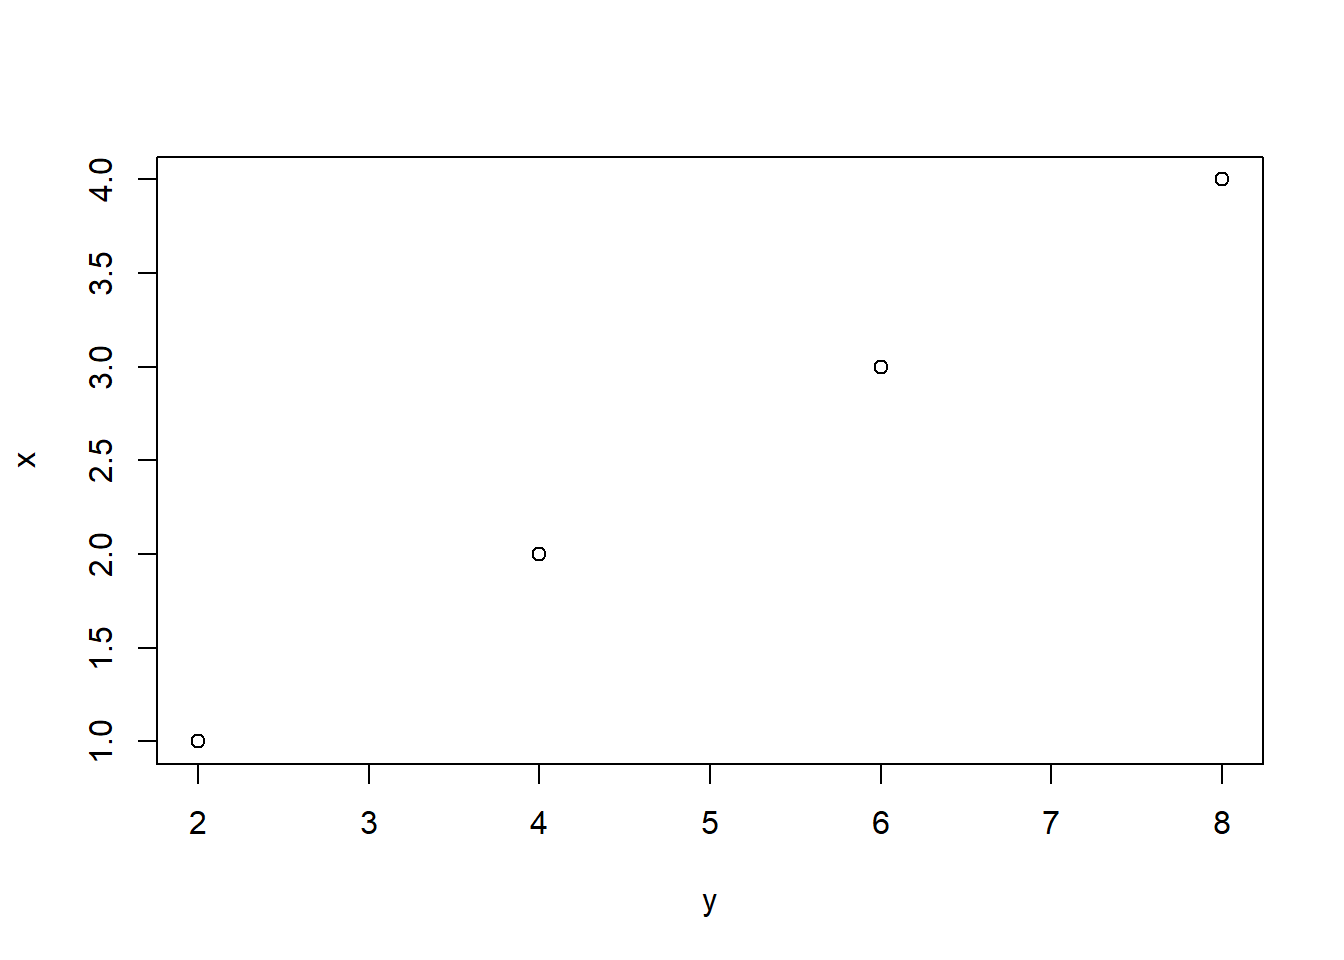
\includegraphics{Lab-3_files/figure-latex/unnamed-chunk-9-1.pdf} It
would be hard to guess a correlation by just looking at this data. There
are only 15 points, but we can tell they are not all in the same space,
nor are they all randomly dispersed. So if we \emph{had} to take a
guess, we could assume that a slight correlation could be prsent.

Let us take a look at a data set with some meaning and more data points.

\begin{Shaded}
\begin{Highlighting}[]
\KeywordTok{plot}\NormalTok{(cars}\OperatorTok{$}\NormalTok{speed}\OperatorTok{~}\NormalTok{cars}\OperatorTok{$}\NormalTok{dist, }\DataTypeTok{xlab=}\StringTok{"Distance"}\NormalTok{,}\DataTypeTok{ylab =} \StringTok{"Speed"}\NormalTok{,}\DataTypeTok{main=}\StringTok{"Distance vs. Speed"}\NormalTok{, }\DataTypeTok{sub =} \StringTok{"r = .81"}\NormalTok{)}
\end{Highlighting}
\end{Shaded}

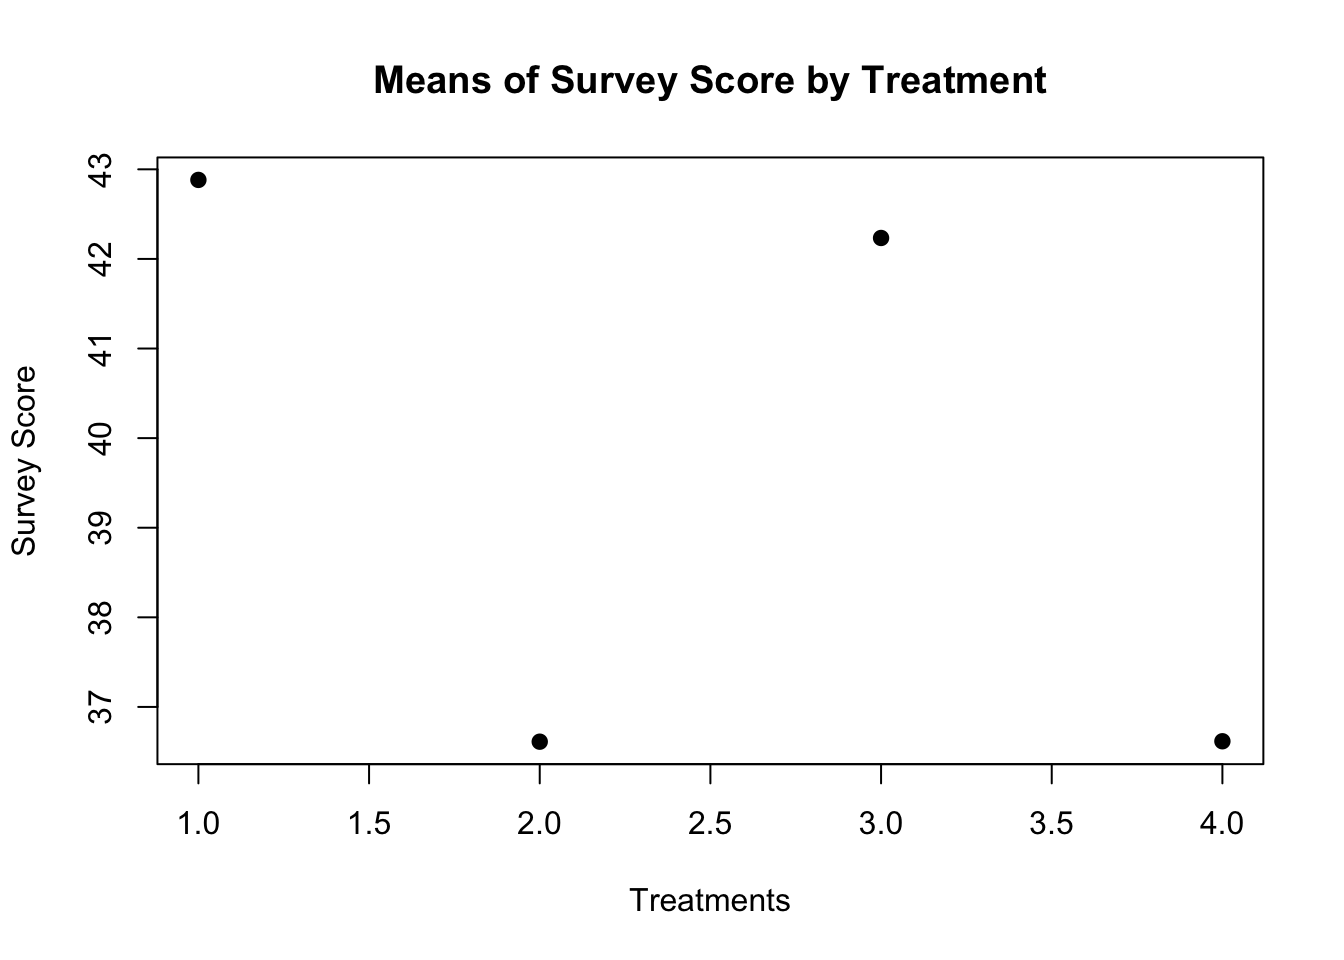
\includegraphics{Lab-3_files/figure-latex/unnamed-chunk-10-1.pdf}

\begin{Shaded}
\begin{Highlighting}[]
\KeywordTok{cor}\NormalTok{(cars}\OperatorTok{$}\NormalTok{speed,cars}\OperatorTok{$}\NormalTok{dist)}
\end{Highlighting}
\end{Shaded}

\begin{verbatim}
## [1] 0.8068949
\end{verbatim}

\subsection{Linear Regression}\label{linear-regression}

Linear regression refers to an equation of the ``best fitting line''
that shows where a line could be placed taht would best explain the
relationship, if any, or your data.

The equation is as follows:

\(\hat{Y} = a + bx\)

Where \(\hat{Y}\) equals the predicted value of Y given X.

In order to find b:

\(b = \frac{n\sum XY -\sum X\sum Y }{n\sum X^2-\sum (X)^2}\) or
\(b = \frac{\sum XY }{\sum X^2}\)

In order to fid a:

\(a = \mathrel{\bar{Y}}-b\mathrel{\bar{X}}\)

Let us work with a sample set of data:

x = 20,25,30,35,40,45,50,55,60,65,70,75,80,85,90,95,100

y =
10.93,11.78,10.97,11.27,11.37,10.31,12.84,12.15,10.86,13.25,12.43,11.70,12.90
12.8,12.82,12.69,12.55

\begin{Shaded}
\begin{Highlighting}[]
\NormalTok{x =}\StringTok{ }\KeywordTok{c}\NormalTok{(}\DecValTok{20}\NormalTok{,}\DecValTok{25}\NormalTok{,}\DecValTok{30}\NormalTok{,}\DecValTok{35}\NormalTok{,}\DecValTok{40}\NormalTok{,}\DecValTok{45}\NormalTok{,}\DecValTok{50}\NormalTok{,}\DecValTok{55}\NormalTok{,}\DecValTok{60}\NormalTok{,}\DecValTok{65}\NormalTok{,}\DecValTok{70}\NormalTok{,}\DecValTok{75}\NormalTok{,}\DecValTok{80}\NormalTok{,}\DecValTok{85}\NormalTok{,}\DecValTok{90}\NormalTok{,}\DecValTok{95}\NormalTok{,}\DecValTok{100}\NormalTok{)}
\NormalTok{y=}\StringTok{ }\KeywordTok{c}\NormalTok{(}\FloatTok{10.93}\NormalTok{,}\FloatTok{11.78}\NormalTok{,}\FloatTok{10.97}\NormalTok{,}\FloatTok{11.27}\NormalTok{,}\FloatTok{11.37}\NormalTok{,}\FloatTok{10.31}\NormalTok{,}\FloatTok{12.84}\NormalTok{,}\FloatTok{12.15}\NormalTok{,}\FloatTok{10.86}\NormalTok{,}\FloatTok{13.25}\NormalTok{,}\FloatTok{12.43}\NormalTok{,}\FloatTok{11.70}\NormalTok{,}\FloatTok{12.90}\NormalTok{,}
 \FloatTok{12.8}\NormalTok{,}\FloatTok{12.82}\NormalTok{,}\FloatTok{12.69}\NormalTok{,}\FloatTok{12.55}\NormalTok{)}
\NormalTok{x}
\end{Highlighting}
\end{Shaded}

\begin{verbatim}
 [1]  20  25  30  35  40  45  50  55  60  65  70  75  80  85  90  95 100
\end{verbatim}

\begin{Shaded}
\begin{Highlighting}[]
\NormalTok{y}
\end{Highlighting}
\end{Shaded}

\begin{verbatim}
 [1] 10.93 11.78 10.97 11.27 11.37 10.31 12.84 12.15 10.86 13.25 12.43
[12] 11.70 12.90 12.80 12.82 12.69 12.55
\end{verbatim}

\begin{enumerate}
\def\labelenumi{\arabic{enumi}.}
\tightlist
\item
  \(n\sum XY -\sum X\sum Y\)
\end{enumerate}

\begin{Shaded}
\begin{Highlighting}[]
\KeywordTok{length}\NormalTok{(x)}
\end{Highlighting}
\end{Shaded}

\begin{verbatim}
## [1] 17
\end{verbatim}

\begin{Shaded}
\begin{Highlighting}[]
\KeywordTok{length}\NormalTok{(y)}
\end{Highlighting}
\end{Shaded}

\begin{verbatim}
## [1] 17
\end{verbatim}

\begin{Shaded}
\begin{Highlighting}[]
\NormalTok{topb=(}\KeywordTok{sum}\NormalTok{(x}\OperatorTok{*}\NormalTok{y))}\OperatorTok{-}\NormalTok{(}\KeywordTok{sum}\NormalTok{(x)}\OperatorTok{*}\NormalTok{(}\KeywordTok{sum}\NormalTok{(y)}\OperatorTok{/}\DecValTok{17}\NormalTok{))}
\NormalTok{topb}
\end{Highlighting}
\end{Shaded}

\begin{verbatim}
[1] 243.25
\end{verbatim}

\begin{enumerate}
\def\labelenumi{\arabic{enumi}.}
\setcounter{enumi}{1}
\tightlist
\item
  \(b = \frac{4135.25}{n\sum X^2-\sum (X)^2}\)
\end{enumerate}

\begin{Shaded}
\begin{Highlighting}[]
\NormalTok{botb=}\StringTok{ }\NormalTok{(}\KeywordTok{sum}\NormalTok{(x}\OperatorTok{^}\DecValTok{2}\NormalTok{))}\OperatorTok{-}\NormalTok{((}\KeywordTok{sum}\NormalTok{(x)}\OperatorTok{^}\DecValTok{2}\NormalTok{)}\OperatorTok{/}\DecValTok{17}\NormalTok{)}
\NormalTok{botb}
\end{Highlighting}
\end{Shaded}

\begin{verbatim}
## [1] 10200
\end{verbatim}

\begin{enumerate}
\def\labelenumi{\arabic{enumi}.}
\setcounter{enumi}{2}
\tightlist
\item
  \(b = \frac{4135.25 }{256}\)
\end{enumerate}

\begin{Shaded}
\begin{Highlighting}[]
\NormalTok{b=topb}\OperatorTok{/}\NormalTok{botb}
\NormalTok{b}
\end{Highlighting}
\end{Shaded}

\begin{verbatim}
## [1] 0.02384804
\end{verbatim}

\(a = \mathrel{\bar{Y}}-b\mathrel{\bar{X}}\)

\begin{Shaded}
\begin{Highlighting}[]
\NormalTok{a=}\KeywordTok{mean}\NormalTok{(y)}\OperatorTok{-}\NormalTok{b}\OperatorTok{*}\NormalTok{(}\KeywordTok{mean}\NormalTok{(x))}
\NormalTok{a}
\end{Highlighting}
\end{Shaded}

\begin{verbatim}
## [1] 10.54676
\end{verbatim}

\(\frac{\sum(X-\mathrel{\bar{X}}^2)\sum(Y-\mathrel{\bar{Y}}^2)}{\sum(X-\mathrel{\bar{X}}\)

\begin{Shaded}
\begin{Highlighting}[]
\NormalTok{ssxy=}\KeywordTok{sum}\NormalTok{((x}\OperatorTok{-}\KeywordTok{mean}\NormalTok{(x))}\OperatorTok{*}\NormalTok{(y}\OperatorTok{-}\KeywordTok{mean}\NormalTok{(y)))}
\NormalTok{ssxy}
\end{Highlighting}
\end{Shaded}

\begin{verbatim}
## [1] 243.25
\end{verbatim}

\begin{Shaded}
\begin{Highlighting}[]
\NormalTok{ssx=}\KeywordTok{sum}\NormalTok{((x }\OperatorTok{-}\StringTok{ }\KeywordTok{mean}\NormalTok{(x))}\OperatorTok{^}\DecValTok{2}\NormalTok{)}
\NormalTok{ssx}
\end{Highlighting}
\end{Shaded}

\begin{verbatim}
## [1] 10200
\end{verbatim}

\(\frac{243.25}{10,200}\)

\begin{Shaded}
\begin{Highlighting}[]
\NormalTok{b =}\StringTok{ }\NormalTok{(ssxy}\OperatorTok{/}\NormalTok{ssx)}
\NormalTok{b =}\StringTok{ }\KeywordTok{round}\NormalTok{(b,}\DataTypeTok{digits=}\DecValTok{4}\NormalTok{)}
\NormalTok{b}
\end{Highlighting}
\end{Shaded}

\begin{verbatim}
## [1] 0.0238
\end{verbatim}

\begin{Shaded}
\begin{Highlighting}[]
\NormalTok{a=(}\KeywordTok{mean}\NormalTok{(y))}\OperatorTok{-}\NormalTok{(b}\OperatorTok{*}\NormalTok{(}\KeywordTok{mean}\NormalTok{(x)))}
\NormalTok{a}
\end{Highlighting}
\end{Shaded}

\begin{verbatim}
## [1] 10.54965
\end{verbatim}

\(\hat{Y} = 10.546 + .0238x\)

\begin{Shaded}
\begin{Highlighting}[]
\NormalTok{xy.mod<-}\KeywordTok{lm}\NormalTok{(y}\OperatorTok{~}\NormalTok{x)}
\NormalTok{xy.mod =}\StringTok{ }\KeywordTok{summary}\NormalTok{(xy.mod)}
\NormalTok{xy.mod}
\end{Highlighting}
\end{Shaded}

\begin{verbatim}

Call:
lm(formula = y ~ x)

Residuals:
     Min       1Q   Median       3Q      Max 
-1.30993 -0.29221 -0.09373  0.29159  1.15311 

Coefficients:
             Estimate Std. Error t value Pr(>|t|)    
(Intercept) 10.546765   0.438253  24.065 2.13e-13 ***
x            0.023848   0.006762   3.527  0.00305 ** 
---
Signif. codes:  0 '***' 0.001 '**' 0.01 '*' 0.05 '.' 0.1 ' ' 1

Residual standard error: 0.683 on 15 degrees of freedom
Multiple R-squared:  0.4533,    Adjusted R-squared:  0.4168 
F-statistic: 12.44 on 1 and 15 DF,  p-value: 0.003052
\end{verbatim}


\end{document}
